\documentclass[a4paper,10pt]{report}
\usepackage{amsmath}
\usepackage{amssymb}
\usepackage{amsfonts}
\usepackage{epstopdf}
\usepackage{epsfig}
\usepackage{textcomp}
\usepackage{inputenc}
\usepackage{fontenc}
\usepackage{graphicx}
\usepackage{color}
\usepackage{breqn}
\usepackage{sectsty}
\usepackage{natbib}
\usepackage{fullpage}
\usepackage{inputenc}
\usepackage{etoolbox}
\usepackage{hyperref}
\usepackage{subfigure}

\begin{document}

\begin{figure}[!htb]
  \centering
    \subfigure[Score]
    {
      \centering
        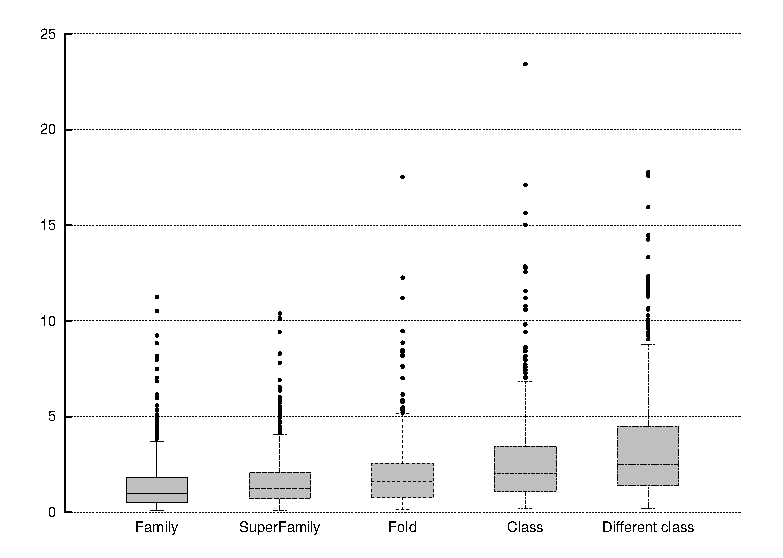
\includegraphics[width=0.45\textwidth]{fig/histograms.boxplot.score0.eps}
        \label{fig:score0}
    }
    \hspace{0.5cm}
    \subfigure[Avg. score]
    {
        \centering
        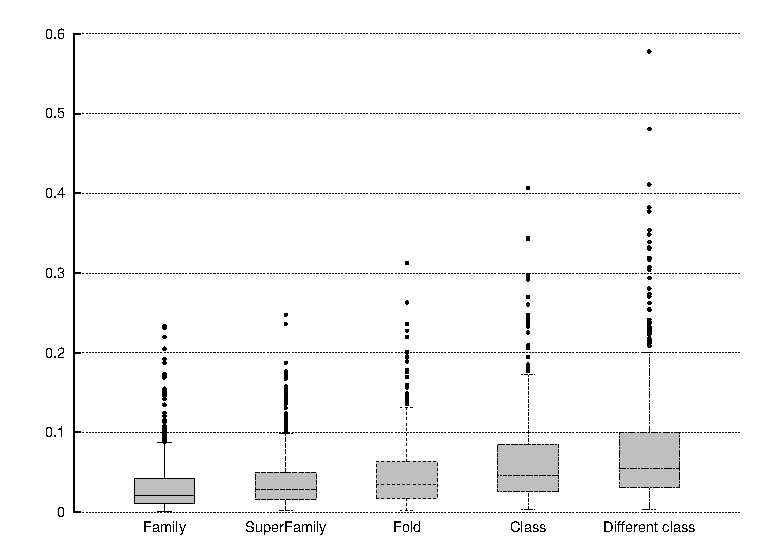
\includegraphics[width=0.45\textwidth]{fig/histograms.boxplot.avg.score0.eps}
        \label{fig:avg_score0}
    }
    \caption{Using the difference in global histogram values (492 pivots): $\sum_{r} H_a(r) - H_b(r)$}
    \label{fig:score0_boxplot}
\end{figure}

\begin{figure}[!htb]
  \centering
    \subfigure[Score]
    {
      \centering
        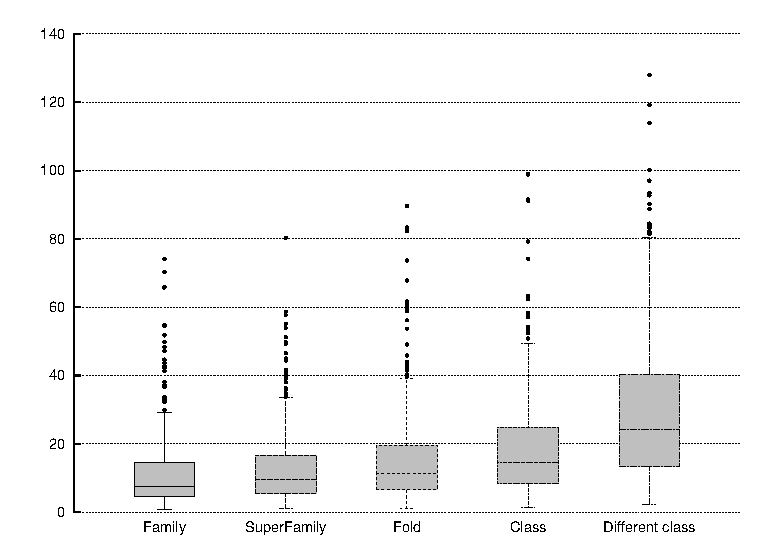
\includegraphics[width=0.45\textwidth]{fig/histograms.boxplot.score1.eps}
        \label{fig:score1}
    }
    \hspace{0.5cm}
    \subfigure[Avg. score]
    {
        \centering
        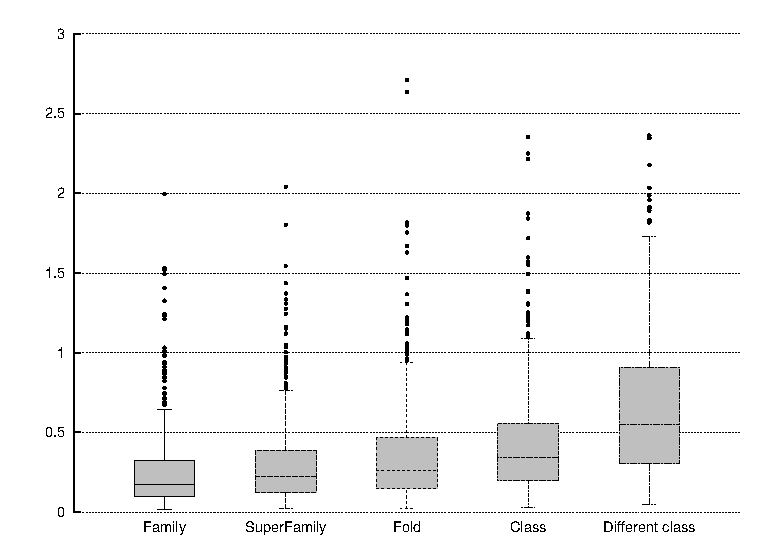
\includegraphics[width=0.45\textwidth]{fig/histograms.boxplot.avg.score1.eps}
        \label{fig:avg_score1}
    }
    \caption{Using the difference in normalized global histogram values (492 pivots): $\sum_{r} \frac{H_a(r)}{\Delta l_1} - \frac{H_b(r)}{\Delta l_2}$}
    \label{fig:score1_boxplot}
\end{figure}

\newpage

\begin{figure}[!htb]
  \centering
    \subfigure[Class A (with $dr = 1$)]
    {
      \centering
        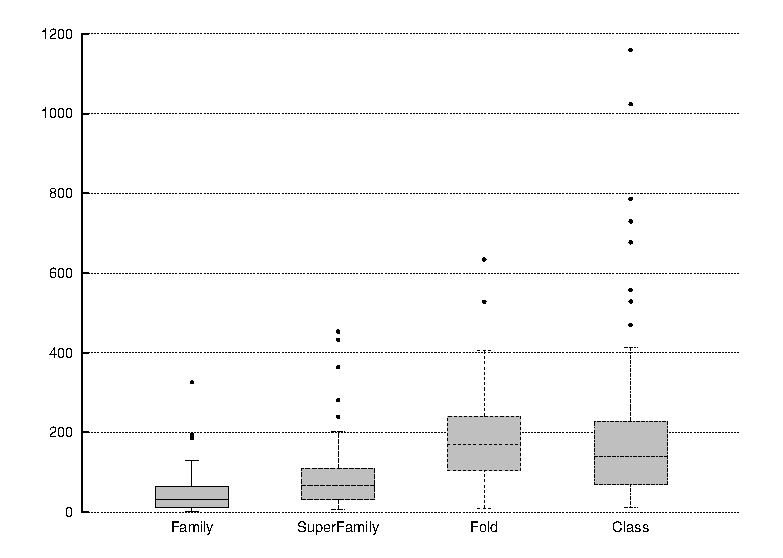
\includegraphics[width=0.45\textwidth]{fig/histograms.boxplot.domains-a.1.eps}
        \label{fig:class_a_dr_1}
    }
    \hspace{0.5cm}
    \subfigure[Class B (with $dr = 1$)]
    {
        \centering
        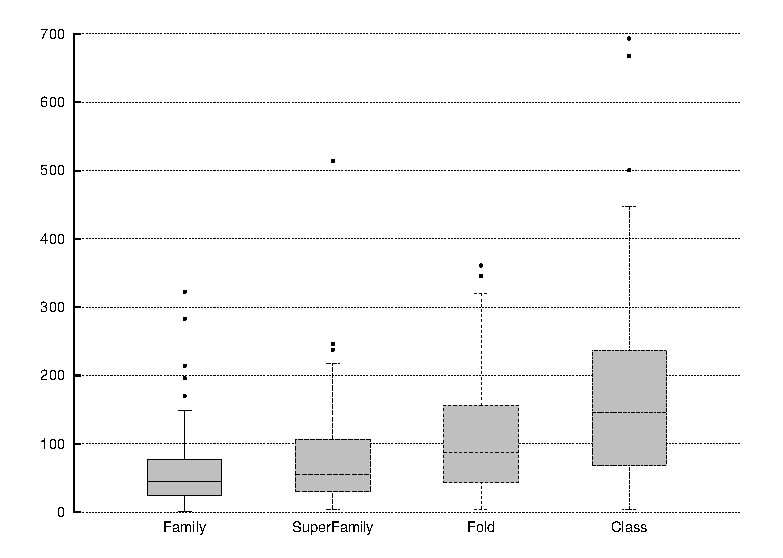
\includegraphics[width=0.45\textwidth]{fig/histograms.boxplot.domains-b.1.eps}
        \label{fig:class_b_dr_1}
    }
    %\caption{Comparison of normalized global histograms}
    \label{fig:class_a_b_dr_1}
\end{figure}

\begin{figure}[!htb]
  \centering
    \subfigure[Class A (with $dr = 5$)]
    {
      \centering
        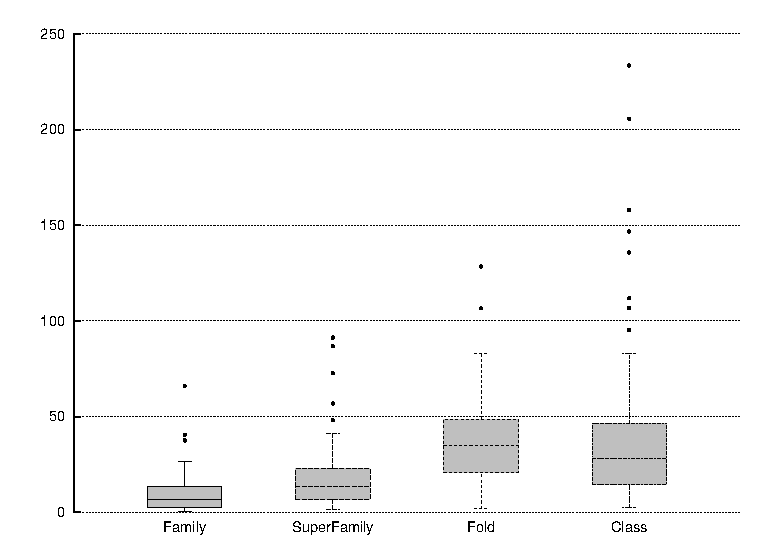
\includegraphics[width=0.45\textwidth]{fig/histograms.boxplot.domains-a.5.eps}
        \label{fig:class_a_dr_5}
    }
    \hspace{0.5cm}
    \subfigure[Class B (with $dr = 5$)]
    {
        \centering
        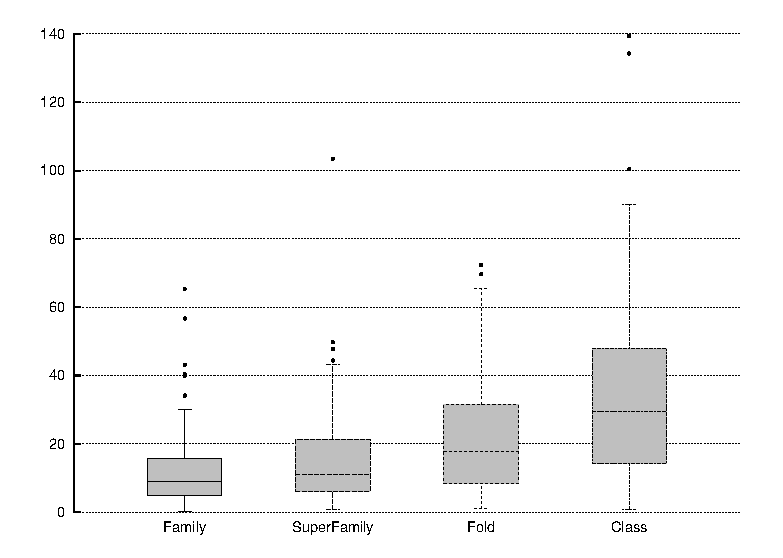
\includegraphics[width=0.45\textwidth]{fig/histograms.boxplot.domains-b.5.eps}
        \label{fig:class_b_dr_5}
    }
    %\caption{Comparison of normalized global histograms}
    \label{fig:class_a_b_dr_5}
\end{figure}

\begin{figure}[!htb]
  \centering
    \subfigure[Class A (with $dr = 10$)]
    {
      \centering
        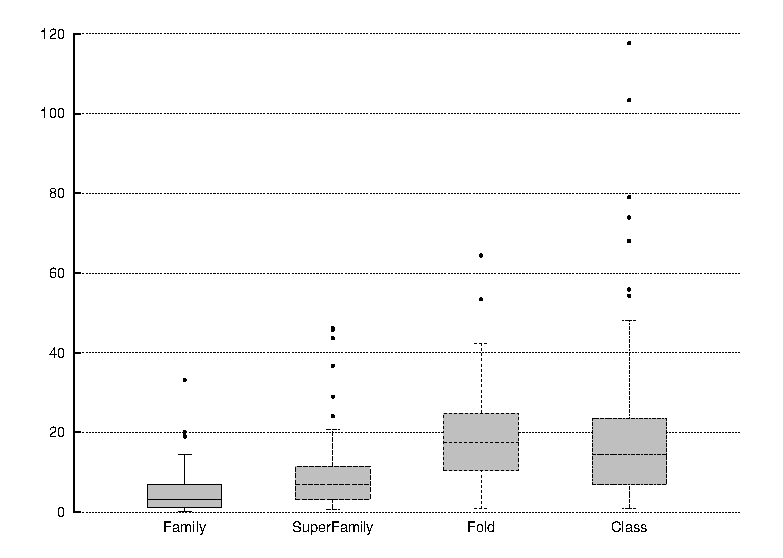
\includegraphics[width=0.45\textwidth]{fig/histograms.boxplot.domains-a.10.eps}
        \label{fig:class_a_dr_10}
    }
    \hspace{0.5cm}
    \subfigure[Class B (with $dr = 10$)]
    {
        \centering
        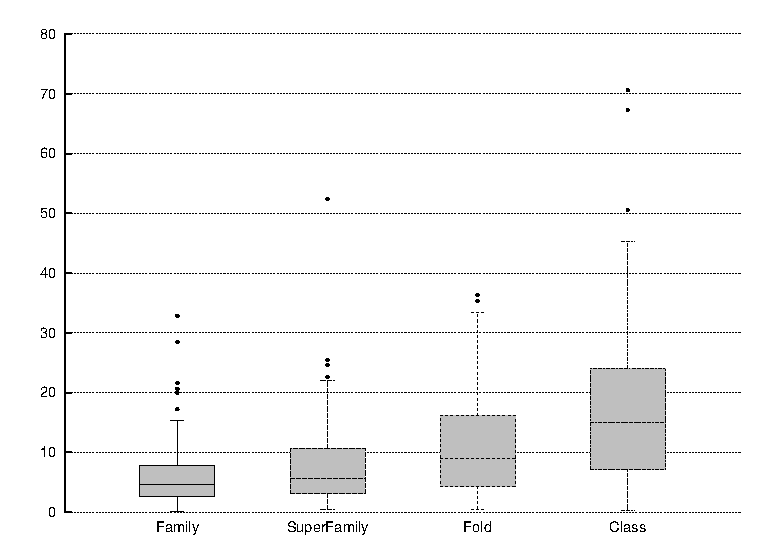
\includegraphics[width=0.45\textwidth]{fig/histograms.boxplot.domains-b.10.eps}
        \label{fig:class_b_dr_10}
    }
    \caption{Comparison of normalized global histograms for classes A and B (100 pivots)}
    \label{fig:class_a_b_dr_10}
\end{figure}

\begin{figure}[!htb]
  \centering
    \subfigure[Class C (with $dr = 5$)]
    {
      \centering
        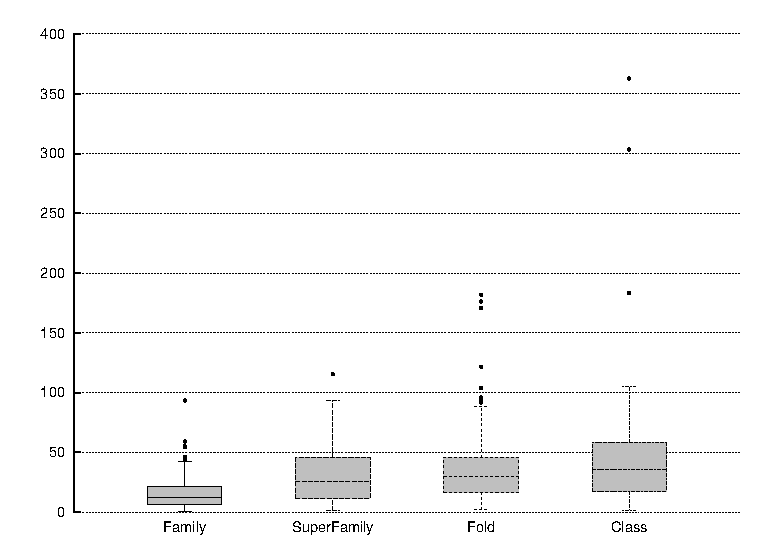
\includegraphics[width=0.45\textwidth]{fig/histograms.boxplot.domains-c.5.eps}
        \label{fig:class_c_dr_10}
    }
    \hspace{0.5cm}
    \subfigure[Class C (with $dr = 10$)]
    {
        \centering
        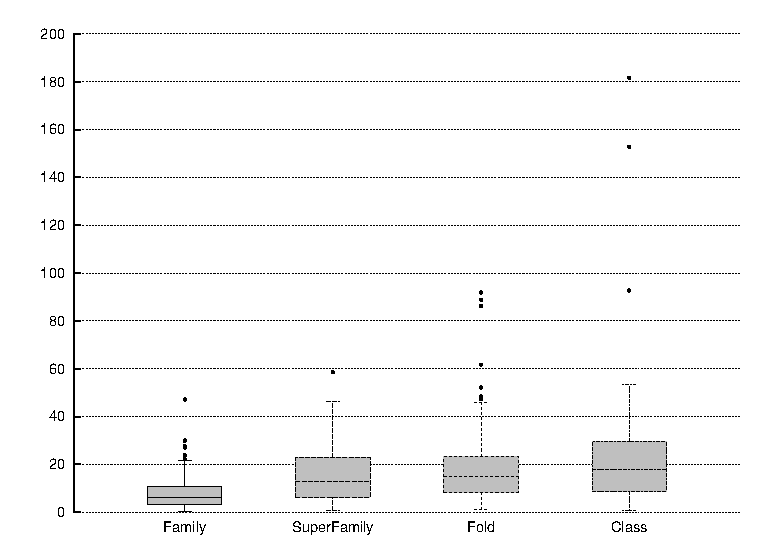
\includegraphics[width=0.45\textwidth]{fig/histograms.boxplot.domains-c.10.eps}
        \label{fig:class_c_dr_10}
    }
    \caption{Comparison of normalized global histograms for class C (100 pivots)}
    \label{fig:class_c_dr_5_10}
\end{figure}

\begin{figure}[!htb]
\centering
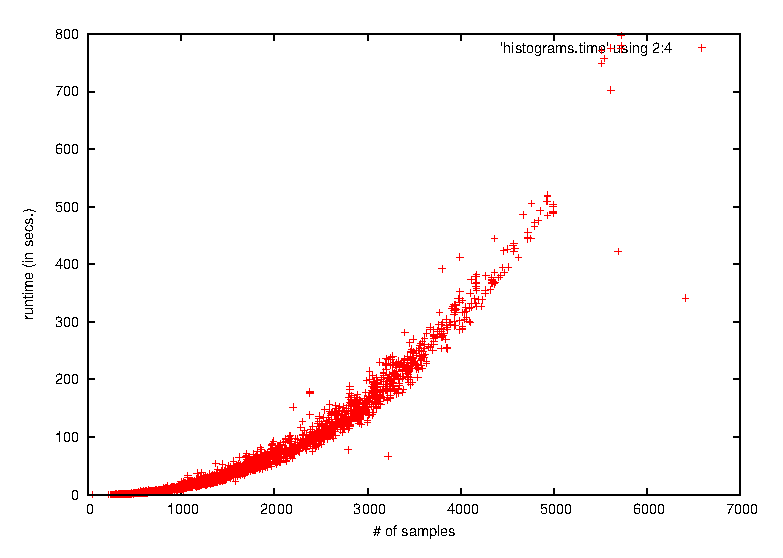
\includegraphics[scale=1.0]{fig/runtime.eps}
\caption{Plot of runtime ($dr = 1$)}
\label{fig:runtime}
\end{figure}
\end{document}

